\documentclass[12pt]{article}
\usepackage[utf8]{inputenc}
\usepackage[margin=1in]{geometry}
\usepackage{tabu}
\usepackage{graphicx}
\usepackage{hyperref}
\usepackage{pdfpages}

\title{Smallpond Architecture Reference Manual}
\author{Zachary Salim, Dominique Hickson,\\ Andrew Balys, Justin Charlong}
\date{Fall Semester 2017}


%MADE PARAGRAPH ANOTHER SECTION LEVEL
%MADE PARAGRAPH ANOTHER SECTION LEVEL
%\makeatletter
%\renewcommand\paragraph{\@startsection{paragraph}{4}{\z@}%
%            {-2.5ex\@plus -1ex \@minus -.25ex}%
%            {1.25ex \@plus .25ex}%
%            {\normalfont\normalsize\bfseries}}
            
%\renewcommand\paragraph{\@startsection{paragraph}{4}{\z@}%
%            {-2.5ex\@plus -1ex \@minus -.25ex}%
%            {1.25ex \@plus .25ex}%
%            {\normalfont\normalsize\bfseries}}
%\makeatother

%SETS THE SECTION NUMBER DEPTH
%SETS TABLE OF CONTENTS DEPTH
%\setcounter{secnumdepth}{5} % how many sectioning levels to assign numbers to
%\setcounter{tocdepth}{5}    % how many sectioning levels to show in ToC

\newcommand{\aTypeInstruction}[5]
{%Numbers above the instruction layout. DO NOT CHANGE
    \hspace{1.6cm}31 \hspace{1.15cm}26 \hspace{.04cm}25 \hspace{.8cm}21 \hspace{.04cm}20 \hspace{.8cm}16 \hspace{.04cm}15 \hspace{.8cm}11 \hspace{.04cm}10 \hspace{.275cm}9 \hspace{.275cm}8 \hspace{1.175cm}4 \hspace{.04cm}3 \hspace{1.25cm}0
    \vspace{-.25cm}
    %Start of the instruction layout table
    \begin{center}
        \begin{tabular}{ |p{1.8cm}|p{1.5cm}|p{1.5cm}|p{1.5cm}|p{0.3cm}|p{0.3cm}|p{1.5cm}|p{1.5cm}| }
            \hline
            \textbf{Inst.} & \textbf{RD}& \textbf{RS1} & \textbf{RS2} & \textbf{S} & \textbf{C} & Unused & \textbf{Cond.}\\
            \hline
            #1 & 25:21 & 20:16 & 15:11 & 10 & 9 & 8:4 &3:0\\
            \hline
        \end{tabular}
    \end{center}
    %End of instruction layout table
    
    \noindent
    \paragraph{Usage}
    \begin{flushleft}
    #2\\
    \end{flushleft}
    
    \paragraph{Syntax}
    \begin{flushleft}
    #3\{cond\}\{S\}\{C\} RD, RS1, RS2\\
    \vspace{1em}        %Gives new line
    where:\\
    \vspace{1em}
    \{cond\}    \hspace{2em} Is the condition under which the instruction is executed. To see a list of\\
                \hspace{5.4em} conditions see page . If \{cond\} is omitted the AL (always) condition is used.\\
    \vspace{1em}    
    S       \hspace{4.5em} Causes the S bit (bit[25]) to be set to a 1. This specified that the instruction\\
            \hspace{5.4em} will update the CPSR. If S is omitted then the S bit (bit[25]) is set to 0 and\\
            \hspace{5.4em} the CPSR is not updated.\\
    \vspace{1em}    
    C       \hspace{4.5em} Causes the C bit (bit[24]) to be set to a 1. This specified that the instruction\\
            \hspace{5.4em} will increment the counter. If C is omitted then the C bit (bit[24]) is set to 0\\
            \hspace{5.4em} and the counter will not be incremented.\\
    \vspace{1em}
    RD  \hspace{3.6em} Destination register of the instruction.\\
    \vspace{1em}
    RS1  \hspace{3.35em} Source register 1 of the instruction.\\
    \vspace{1em}
    RS2  \hspace{3.35em} Source register 2 of the instruction.\\
    \end{flushleft}
    
    \paragraph{Example}
    \begin{flushleft}
    % 1Short example of use
    % Ex: To LSR a value in register Rx by a value in register Ry and store the result into register Rz.
    #4\\
    \vspace{1em}
    % Example of instruction syntax
    % LSR Rz, Rx, Ry
    #5
    \end{flushleft}
    }
    
\newcommand{\iTypeInstruction}[5]
{%Numbers above the instruction layout. DO NOT CHANGE
    \hspace{1.6cm}31 \hspace{1.15cm}26 \hspace{.05cm}25 \hspace{.8cm}21 \hspace{.05cm}20 \hspace{.8cm}16 \hspace{.05cm}15 \hspace{6.4cm}0
    \vspace{-.25cm}
    %Start of the instruction layout table
    \begin{center}
        \begin{tabular}{ |p{1.8cm}|p{1.5cm}|p{1.5cm}|p{6.8cm}| }
            \hline
            \textbf{Inst.} & \textbf{RD} &  \textbf{RS} & \textbf{Immediate}\\
            \hline
            %Instruction number
            #1 & 25:21 & 20:16 &15:0\\
            \hline
        \end{tabular}
    \end{center}
    %End of instruction layout table
    
    \noindent
    % The ADDI instruction adds the value of RS to the value of a 16 %bit immediate and stores the result in register RD. 
    \paragraph{Usage}
    \begin{flushleft}
    #2
    \end{flushleft}
    
    \paragraph{Syntax}
    \begin{flushleft}
    #3 RD, RS1, \#imm.\\
    \vspace{1em}        %Gives new line
    where:\\
    \vspace{1em}
    RD  \hspace{3.6em} Destination register of the instruction.\\
    \vspace{1em}
    RS1  \hspace{3.35em} Source register of the instruction.\\
    \vspace{1em}
    \#imm.  \hspace{1.8em} The immediate value of the instruction, must be capable of being represented\\             \hspace{5.4em} in 16 bits. The syntax to represent a decimal number is as follows:\\
            \hspace{5.4em} \#decimal\_number, i.e. \#1 to represent a one. The syntax to represent a\\
            \hspace{5.4em} hexadecimal number is as follows: \#0xhexadecimal\_number, i.e. \#0x3F2A \\
            \hspace{5.4em} to represent a hexadecimal 0x3F2A or \#0xA to represent 0x000A.\\
    \end{flushleft}
    
    \paragraph{Example}
    \begin{flushleft}
    %To increment a value in register Rx by an immediate of 1.\\
    #4\\
    \vspace{1em}
    %ADDI Rx, Rx, \#1
    #5
    \end{flushleft}}
    
\newcommand{\bTypeInstruction}[5]
{%Numbers above the instruction layout. DO NOT CHANGE
    \hspace{1.6cm}31 \hspace{1.15cm}26 \hspace{.08cm}25 \hspace{.08cm}24 \hspace{.45cm}22 \hspace{.05cm}19 \hspace{6.0cm}4 \hspace{.04cm}3 \hspace{1.25cm}0
    \vspace{-.25cm}
    %Start of the instruction layout table
    \begin{center}
        \begin{tabular}{|p{1.8cm}|p{.3cm}|p{1.1cm}|p{6.5cm}|p{1.5cm}| }
            \hline
            \textbf{Inst.} & \textbf{C} & unused &\textbf{Immediate}&\textbf{Cond.}\\
            \hline
            #1& 25  & 24:21 &19:4 &3:0\\
            \hline
        \end{tabular}
    \end{center}
    %End of instruction layout table
    
    \noindent
    %The branch instruction allows to conditionally relocate the %program counter to a location above or below the instruction.
    #2
    
    \paragraph{Syntax}
    \begin{flushleft}
    #3\{cond\}\{C\} target\_address\\
    \vspace{1em}        %Gives new line
    where:\\
    \vspace{1em}
    C       \hspace{4.5em} Causes the C bit (bit[24]) to be set to a 1. This specified that the instruction\\
            \hspace{5.4em} will increment the counter. If C is omitted then the C bit (bit[24]) is set to 0\\
            \hspace{5.4em} and the counter will not be incremented.\\
    \vspace{1em}
    \#imm.  \hspace{1.8em} The immediate value of the instruction, must be capable of being represented\\              \hspace{5.4em} in 16 bits. The syntax to represent a decimal number is as follows:\\
            \hspace{5.4em} \#decimal\_number, i.e. \#1 to represent a one. The syntax to represent a\\
            \hspace{5.4em} hexadecimal number is as follows: \#0xhexadecimal\_number, i.e. \#0x3F2A \\
            \hspace{5.4em} to represent a hexadecimal 0x3F2A or \#0xA to represent 0x000A.\\
    \vspace{1em}
    \{cond\}    \hspace{2em} Is the condition under which the instruction is executed. To see a list of\\
                \hspace{5.4em} conditions see page . If \{cond\} is omitted the AL (always) condition is used.\\
    \end{flushleft}
    
    \paragraph{Usage}
    \begin{flushleft}
    %To conditionally change the PC \\
    #4\\
    \end{flushleft}
    \paragraph{Example}
    \begin{flushleft}
    %Instruction Syntax
    #5
    \end{flushleft}}

%SETSUP THE HYPERLINK COLORS
\hypersetup{
    colorlinks=true,
    linkcolor=blue,
    filecolor=magenta,      
    urlcolor=cyan,
}


\begin{document}

\maketitle

\begin{center}
    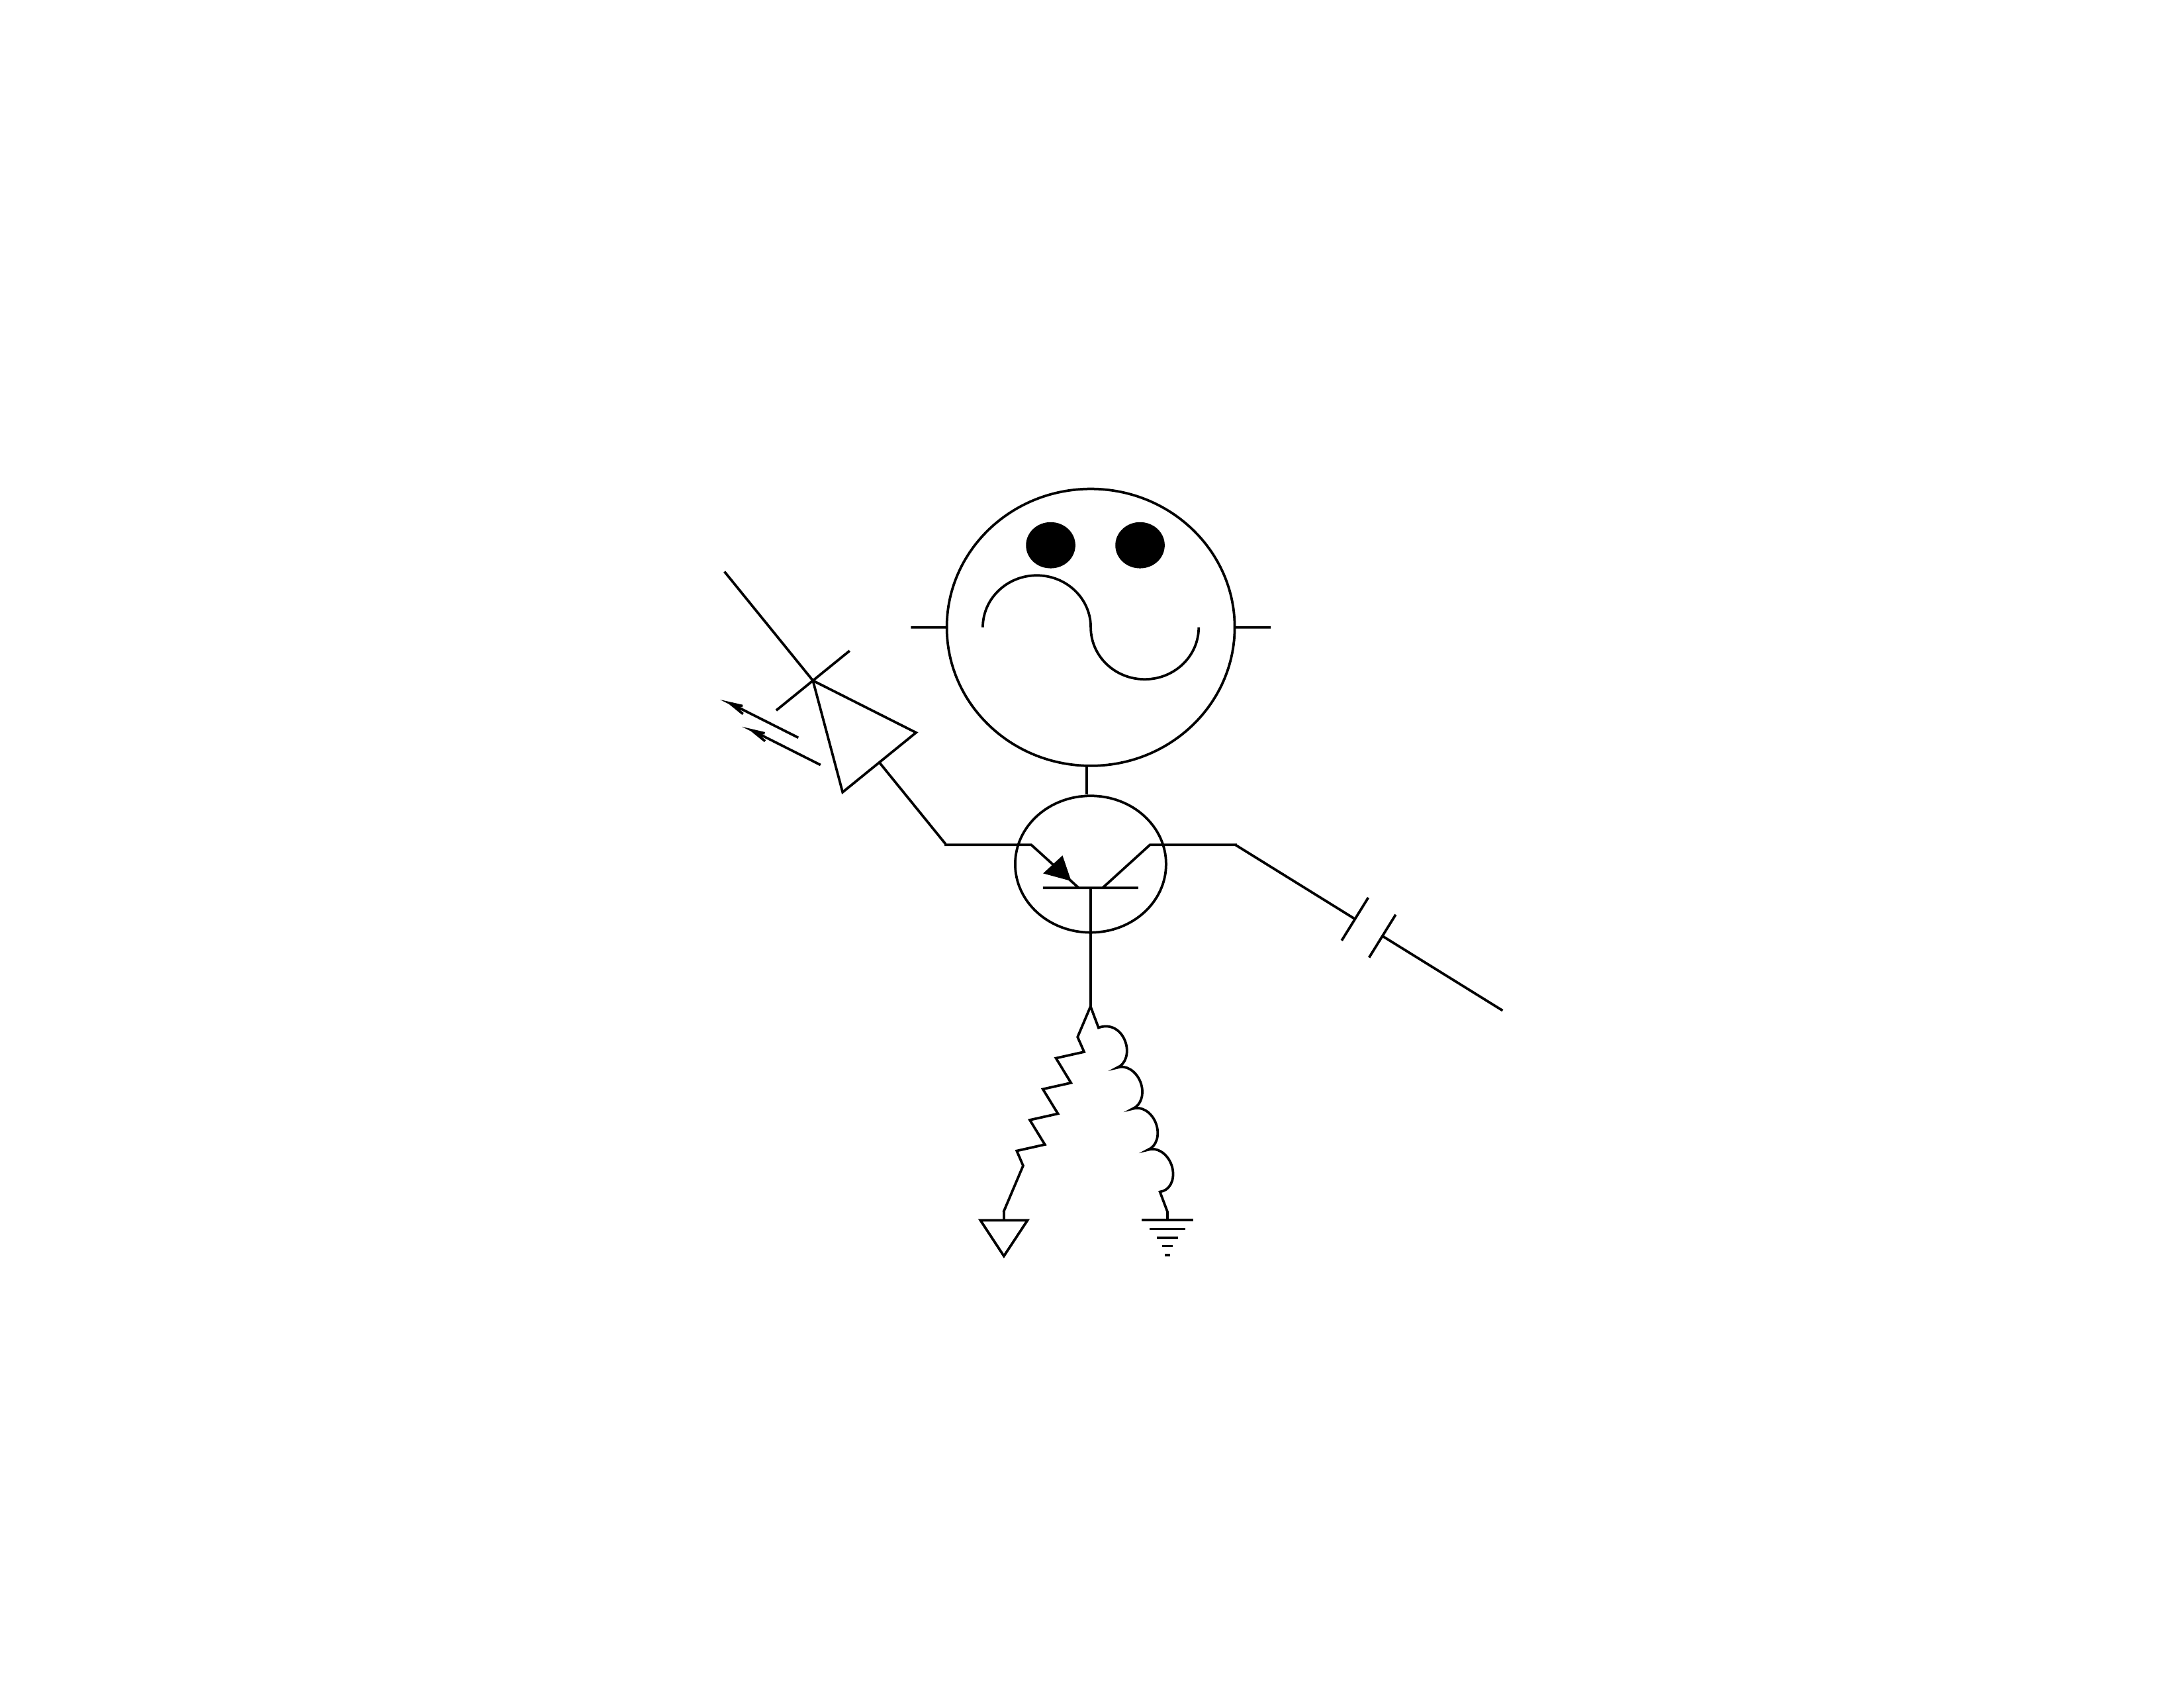
\includegraphics[width=15cm, height=11.6cm]{Volty.png}
\end{center}

\newpage
\tableofcontents

\newpage
\section{Introduction}
Smallpond is a fully custom 32 bit RISC CPU designed by Zachary Salim, Dominique Hickson, Andrew Balys and Justin Charlong under the guidance of Dr. Kris Schindler as a part of CSE 490 Computer Architecture in the Fall of 2017. This architecture contains our favorite features from the MIPS 2000/3000 and ARM 7 TDMI processors as well as some new features including, but not limited to, multiple instruction types, 32 general purpose registers, condition codes for most instructions, a CPSR and many more.

\section{Purpose}
Smallpond was developed as a way to provide the Computer Architecture (CSE 490) and the Compilers (CSE 443) students a way to work together. This architecture will be the target for the compiler's students work. The hope is for this architecture to be used in many more courses. Eventually seeing a custom operating system (developed by the OS students), Computer Organization (CSE 341) students studying and writing assembly for Smallpond, Intro to Microprocessors (CSE 379) students writing large assembly programs and studying/discussing the features and possible improvements of Smallpond, and finally Computer Architecture (CSE 490) students implementing improvements via new revisions of the architecture. 

\section{Naming}
You are probably wondering "Why Smallpond? That doesn't make any sense at all for an architecture name." There is a meaning behind the name and it will all make sense in a moment. To start, credit for the name goes to Jeremy Pettrot and Andrew Balys. They each came up with half of the name itself. The idea came from Intel's naming scheme for their Skylake, Kabylake and Coffelake CPU lines. All they did was change the first half of the word for each new generation. We wanted a name that could do the same thing. This is when Jeremy suggested "pond" because this is a RISC architecture (smaller than CISC) and a pond is smaller than a lake. When Andrew hear about Jeremy's suggestion he suggested "small" because it was our first revision and it could be expanded upon later i.e "Mediumpond" etc.
\newpage

\section{Continuation}
Since I (Zack) own the repository on GitHub I will not be able to just pass it on to the next round of students. I would like to keep the working first revision of Smallpond protected in it's final state in that repository. My idea for future expansion and addition to the repository is to fork of the existing one as a new revision e.g "Smallpond Rev B". Small feature additions would only merit a revision increase (A to B, B to C), whereas a large (pipe-lining the architecture) could be a new generation ("Mediumpond").

    \section{Potential Future Features}
    Here are some of the potential features (in no particular order) we thought might be good additions to Smallpond in the future.\\
    \begin{itemize}
        \item Pipe-lining
        \item UART communication
        \item Interrupts
        \item Exceptions
        \item Timers
        \item Basic Cache using fast-block RAM on FPGA
        \item GPU co-processor (another board or on-chip)
        \item Multi-Core CPU
    \end{itemize}
    
\newpage

\section{Smallpond Programming Model}
    \subsection{Data Types}
        \textbf{Byte} \hspace{2cm}8 bits\\
        \textbf{Halfword} \hspace{1.05cm}16 Bits\\
        \textbf{Word} \hspace{1.8cm}32 Bits\\
        %\vspace{1em}
        
       \noindent\rule{1.5cm}{0.3pt}Note\rule{1.5cm}{0.3pt}
       
       \begin{itemize}
           \item Unless specified as \textit{unsigned} integer in the range 0 to 2\textsuperscript{N}-1, the N-bit value will be considered a signed integer in the range, -2\textsuperscript{N-1} to +2\textsuperscript{N-1}, using two's complement format.
           
           \item Load and store operations can transfer bytes, halfwords and words to and from memory,
            automatically zero-extending or sign-extending bytes or halfwords as they are loaded.
    
           \item Smallpond instructions are exactly one word (and are aligned on a four-byte boundary).
           
           \item All data operations , A type, are performed in word quantities
       \end{itemize}
   
   \noindent\rule{4cm}{0.3pt}
   
   \subsection{Condition Codes}   \begin{center}
   \begin{tabular}{|p{1.2cm}|p{1.2cm}|p{5.0cm}|p{7.0cm}|}
        \hline
        \textbf{Cond.} & \textbf{Code} & \textbf{Meaning} & \textbf{cond. Flag State}\\
        \hline
        AL & 0000 & Always & Unconditional\\
        \hline
        EQ & 0001 & Equal & Z set\\
        \hline
        NE & 0010 & Not equal & Z clear\\
        \hline
        CA & 0011 & Carry set & C set\\
        \hline
        CC & 0100 & Carry clear & C clear\\
        \hline
        NG & 0101 & Negative & N set\\
        \hline
        PZ & 0110 & Positive or zero & N clear\\
        \hline
        VS & 0111 & Overflow set & V set\\
        \hline
        VC & 1000 & Overflow clear & V clear\\
        \hline
        HI & 1001 & Unsigned higher & C set and Z clear\\
        \hline
        LS & 1010 & Unsigned lower or same & C clear or Z set\\
        \hline
        GE & 1011 & Signed greater than or equal & N set and V set,\newline
        or N clear and V clear (N==V)\\
        \hline
        LT & 1100 & Signed less than & N set and V clear,\newline
        or N clear and V set (N!=V)\\
        \hline
        GT & 1101 & Signed greater than & Z clear, and either N set and V set, or\newline
        N clear and V clear (Z==0,N==V)\\
        \hline
        LE & 1110 & Signed less than or equal & Z set, or either N set and V clear, or\newline
        N clear and V set (Z==1 or N!=V)\\
        \hline
   \end{tabular}
   \end{center}
   \newpage
   
   \subsection{Registers and Register Conventions}
   
   There are a total of 32 registers in the Smallpond processor:
   \begin{itemize}
       \item 32 general purpose registers, with a program counter.
       \item  All registers are 32 bits wide.
   \end{itemize}
   
   \begin{center}
   \begin{tabular}{|p{1.6cm}|p{2cm}||p{1.6cm}|p{2cm}|}
        \hline
        \textbf{Register} & \textbf{Use} & \textbf{Register} & \textbf{Use}\\
        \hline
        R0 & 0 & R16 & Saved\\
        \hline
        R1 & Arg\_0 & R17 &Saved\\
        \hline
        R2 & Arg\_1 & R18 &Saved\\
        \hline
        R3 & Arg\_2 & R19 &Pos/Neg\\
        \hline
        R4 & Arg\_3 & R20 &Neg/Pos\\
        \hline
        R5 & Temp & R21 &+ Counter\\
        \hline
        R6 & Temp. & R22 &- Counter\\
        \hline
        R7 & Temp. & R23 &HP\\
        \hline
        R8 & Temp. & R24 &FP\\
        \hline
        R9 & Temp. & R25 &SP\\
        \hline
        R10 & Temp. & R26 &LR\_0\\
        \hline
        R11 & Temp. & R27 &LR\_1\\
        \hline
        R12 & Temp. & R28 &LR\_2\\
        \hline
        R13 & Saved & R29 &LR\_3\\
        \hline
        R14 & Saved & R30 & PC\\
        \hline
        R15 & Saved & R31 & CPSR\\
        \hline
   \end{tabular}
   \end{center}
    
    \subsubsection{Register Zero}
        Register zero (R0) is hardwired to zero (0x00000000). Writing to register zero will have no effect on its contents.
        
    \subsubsection{Argument Registers}
        Registers 1-4 (R1, R2, R3, R4) should be used to pass arguments into and out of routines.
        
    \subsubsection{Temporary Registers}
        Registers 5-12 (R5, R6, R7, R8, R9, R10, R11, R12) are temporary registers (scratch registers). They should be used for general calculations and for storing temporary results. Their contents need not be preserved across routine calls.
        
    \subsubsection{Save Registers}
        Registers 13-18 (R13, R14, R15, R16, R17, R18) are save registers which should be used to save results. These registers' values should be preserved across routine calls. If the values are modified in a routine their values should be returned before exiting the routine.
        
    \subsubsection{2's Complement Pair Registers}
        Registers 19 and 20 (R19, R20) are a positive/negative pair. Any value stored into register 19 will update register 20 with the 2's complement of register 22. Storing to register 20 will update register 22 with the 2's complement of register 20.
        
    \subsubsection{Counter Registers}
        Registers 21 and 22 (R21, R22) are counter registers. Writing a value to either register will write to both registers. Activating the counter through the 'C' flag in a command will increment register 21 by 1, and decrement register 22 by 1.
        
    \subsubsection{Heap Pointer Register}
        Register 23 (R23) is the heap pointer register. It should be maintained as a constant reference to the heap.
        
    \subsubsection{Frame Pointer Register}
        Register 24 (R24) is the frame pointer register. It should be maintained as a constant reference to the stack.
        
    \subsubsection{Stack Pointer Register}
        Register 25 (R25) is the stack pointer register. It should be maintained as a reference to the stack.
        
    \subsubsection{Link Registers}
        Link registers are meant to be used in the order 0 to 3 when storing and from 3 to 0 when restoring. This is only a software convention
        
    \subsubsection{Program Counter Register}
        Register 30 (R30) is the program counter. It contains a reference to the next instruction's address in memory.
        
    \subsubsection{Current Program Status Register}
        \begin{center}
        \begin{tabular}{
        |p{10.6cm}|p{0.3cm}|p{0.3cm}|p{0.3cm}|p{0.3cm}|}
            \hline
            \textbf{Unused} & \textbf{N} & \textbf{Z} & \textbf{C} & \textbf{V}\\
            \hline
            31:4 & 3 & 2 & 1 & 0\\
            \hline
        \end{tabular}
        \end{center}
        \vspace{.5em}
        Register 31 (R31) is the current program status register (CPSR). The CPSR contains information as to the status of the processor. It can be used to make decisions and is referred to by programs which make use of conditions. The 'S' flag in an instruction is used to set the CPSR and update its values based on the instruction's results..
    

\newpage

    \subsection{Instruction Types}
        The Smallpond architecture has 4 instruction types: A type, I type, J type, and B type. The A type instructions utilize up to 2 input registers and output the result into a third register. The I type instructions perform on 1 input register with immediate data and output the result into a second register. The J type instruction is used in conjunction with an immediate to change the program counter. The B type instructions also use immediate data to change the program counter however they can do so conditionally. This section outlines the Smallpond architecture's instructions by instruction type. The four types are outlined below:\\
    
        % R Type
        %Start of the instruction layout table
        \begin{center}
            A type:\\
            \vspace{1em}
            \begin{tabular}{ |p{1.8cm}|p{1.5cm}|p{1.5cm}|p{1.5cm}|p{0.3cm}|p{0.3cm}|p{1.5cm}|p{1.5cm}| }
                \hline
                \textbf{Inst.} & \textbf{RD}& \textbf{RS1} & \textbf{RS2} & \textbf{S} & \textbf{C} & Unused & \textbf{Cond.}\\
                \hline
                31:26& 25:21 & 20:16 & 15:11 & 10 & 9 & 8:4 &3:0\\
                \hline
            \end{tabular}
        \end{center}
        %End of instruction layout table for A type
        
        % Immediate Type
        %Start of the instruction layout table
        \begin{center}
            Immediate type:\\
            \vspace{1em}
            \begin{tabular}{ |p{1.8cm}|p{1.5cm}|p{1.5cm}|p{6.8cm}| }
                \hline
                \textbf{Inst.} & \textbf{RD} &  \textbf{RS1} & \textbf{Immediate}\\
                \hline
                31:26& 25:21 & 20:16 &15:0\\
                \hline
            \end{tabular}
        \end{center}
        %End of instruction layout table for I type
        
        %  Type
        %Start of the instruction layout table
        \begin{center}
            Jump type:\\
            \vspace{1em}
            \begin{tabular}{ |p{1.8cm}|p{10.7cm}| }
                \hline
                \textbf{Inst.} & \textbf{Immediate}\\
                \hline
                31:26& 25:0\\
                \hline
            \end{tabular}
        \end{center}
        %End of instruction layout table for J type
        
        % Branch Type
        %Start of the instruction layout table
        \begin{center}
            Branch type:\\
            \vspace{1em}
            \begin{tabular}{|p{1.8cm}|p{.3cm}|p{1.1cm}|p{6.5cm}|p{1.5cm}| }
                \hline
                \textbf{Inst.} & \textbf{C} & unused &\textbf{Immediate}&\textbf{Cond.}\\
                \hline
                31:26& 25 & 24:20 &19:4 &3:0\\
                \hline
            \end{tabular}
        \end{center}
        %End of instruction layout table for B type
    
%%%%%%%%%%%%%%%%%%%%%%%%%%%%%%%%%%%%%%%%%%%%%%%%%%%%%%%%%%%%%%%%%%%%%%%%%%%%%%%%%%%%%%%%%%
%%%%%%%%%%%%%%%%%%%%%%%%%%%%%%%%%% A TYPE INSTRUCTIONS %%%%%%%%%%%%%%%%%%%%%%%%%%%%%%%%%%%
%%%%%%%%%%%%%%%%%%%%%%%%%%%%%%%%%%%%%%%%%%%%%%%%%%%%%%%%%%%%%%%%%%%%%%%%%%%%%%%%%%%%%%%%%%
\newpage

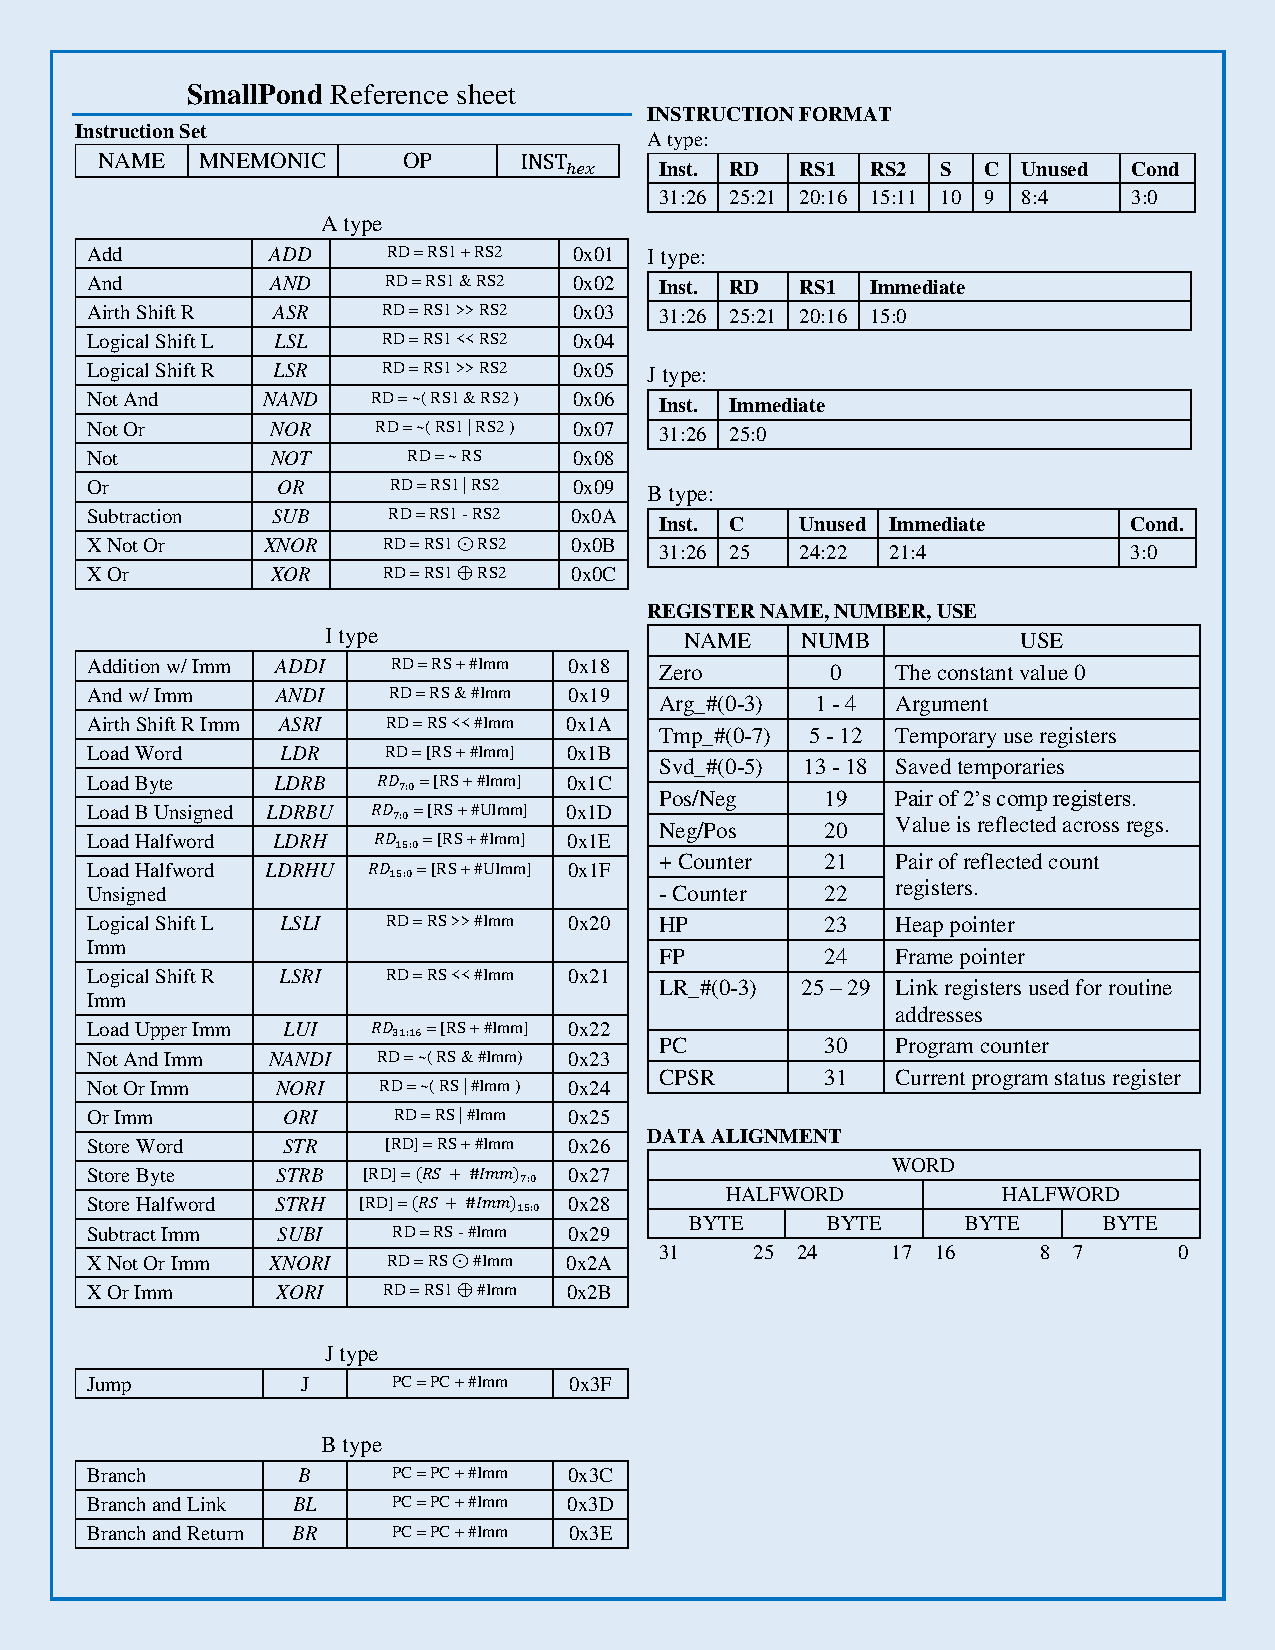
\includepdf[pages={1}]{SmallPond_Reference_sheet.pdf}

\newpage
\section{Smallpond Instruction Set}
    \subsection{A Type}
    
    
    %BEGINNING OF ADD INSTRUCTION   
    
        
        %ADD
        %Title of section
        \subsubsection{Addition (ADD)}
        
        \aTypeInstruction
        {000001}
        {The ADD instruction adds the values stored in the two source registers (RS1 and RS2) and stores the result in the destination register RD.}
        {ADD}
        {Adding the values in Rx and Ry and storing the result in Rz.}
        {ADD Rz, Rx, Ry}
    
    %END OF ADD INSTRUCTION
    
    %BEGINNING OF AND INSTRUCTION  
    
    
        \newpage
        %Title of section
        \subsubsection{And (AND)}
        
        \aTypeInstruction
        {000010}
        {The AND instruction executes a bitwise AND of the values stored in the two source registers (RS1 and RS2) and stores the result in the destination register RD.}
        {AND}
        {Anding the values in Rx and Ry and storing the result in Rz.}
        {AND Rz, Rx, Ry}
       
       
    %END OF AND INSTRUCTION
    
    
    %BEGINNING OF ASR INSTRUCTION  
    
    
        \newpage
        %ASR
        %Title of section
        \subsubsection{Arithmetic Shift Right (ASR)}
        
        \aTypeInstruction
        {000011}
        {The ASR instruction arithmetically right shifts the value stored in RS1 by the value stored in RS2 and stores the result into register RD.}
        {ASR}
        {To ASR a value in register Rx by a value in register Ry and store the result into register Rz.}
        {ASR Rz, Rx, Ry}
       
       
    %END OF ASR
    
       
    %BEGINNING OF LSL INSTRUCTION  
    
    
        \newpage
        %AND
        %Title of section
        \subsubsection{Logical Shift Left (LSL)}
        
        \aTypeInstruction
        {000100}
        {The LSL instruction logically left shifts the value stored in RS1 by the value stored in RS2 and stores the result into register RD.}
        {LSL}
        {To LSL a value in register Rx by a value in register Ry and store the result into register Rz.}
        {LSL Rz, Rx, Ry}
       
    %END OF LSL INSTRUCTION
    
    
    %BEGINNING OF LSR INSTRUCTION  
    
    
        \newpage
        %AND
        %Title of section
        \subsubsection{Logical Shift Right (LSR)}
        
        \aTypeInstruction
        {000101}
        {The LSR instruction logically right shifts the value stored in RS1 by the value stored in RS2 and stores the result into register RD.}
        {LSR}
        {To LSR a value in register Rx by a value in register Ry and store the result into register Rz.}
        {LSR Rz, Rx, Ry}
       
       
    %END OF LSR INSTRUCTION 
    
    
    %BEGINNING OF NAND INSTRUCTION
    
    
        \newpage
        %AND
        %Title of section
        \subsubsection{Not And (NAND)}
        
        \aTypeInstruction
        {000110}
        {The NAND instruction executes a bitwise NAND of the value in RS1 and the value in RS2 and stores the result in register RD.}
        {NAND}
        {To NAND a value in register Rx with a value in register Ry and store the result into Rx.}
        {NAND Rx, Rx, Ry}
        
       
    %END OF NAND INSTRUCTION
    
    
    %BEGINNING OF NOR INSTRUCTION
    
    
        \newpage
        %AND
        %Title of section
        \subsubsection{Not Or (NOR)}
        
        \aTypeInstruction
        {000111}
        {The NOR instruction executes a bitwise NOR of the value in RS1 and the value in RS2 and stores the result in register RD.}
        {NOR}
        {To NOR a value in register Rx with a value in register Ry and store the result into Rx.}
        {NOR Rx, Rx, Ry}
       
    
    %END OF NOR INSTRUCTION
    
    
    %BEGINNING OF NOT INSTRUCTION
    
        \newpage
        %NOT
        %Title of section
        \subsubsection{Not (NOT)}
        
        \aTypeInstruction
        {001000}
        {The NOT instruction executes a bitwise NOT of the value in RS1 and stores the result in register RD.}
        {NOT}
        {To NOT a value in register Rx and store the result into Rx.}
        {NOT Rx, Rx}
       
    %END OF NOT INSTRUCTION
    
    
    %BEGINNING OF OR INSTRUCTION
    
        \newpage
        %OR
        %Title of section
        \subsubsection{Or (OR)}
        
        \aTypeInstruction
        {001001}
        {The OR instruction executes a bitwise OR of the value in RS1 and the value in RS2 and stores the result in register RD.}
        {OR}
        {To OR a value in register Rx with a value in register Ry and store the result into Rx.}
        {OR Rx, Rx, Ry}
        
       
    %END OF OR INSTRUCTION   
    
    
    %BEGINNING OF  INSTRUCTION
    
    
        \newpage
        %
        %Title of section
        \subsubsection{Subtraction (SUB)}
        
        \aTypeInstruction
        {001010}
        {The  instruction subtracts the value of RS2 from the value of RS1 and stores the result in register RD.}
        {}
        {To SUB a value in register Rx from register Ry and store the result into Rz.}
        {SUB Rz, Ry, Rx}
       
       
    %END OF  INSTRUCTION
    
    
    %BEGINNING OF XNOR INSTRUCTION
    
    
        \newpage
        %AND
        %Title of section
        \subsubsection{Exclusive Not Or (XNOR)}
        
        \aTypeInstruction
        {001011}
        {The XNOR instruction executes a bitwise XNOR of the value in RS1 and the value in RS2 and stores the result in register RD.}
        {XNOR}
        {To XNOR a value in register Rx with a value in register Ry and store the result into Rx.}
        {XNOR Rx, Rx, Ry}
        
       
    %END OF XNOR INSTRUCTION
    
    
    %BEGINNING OF XOR INSTRUCTION
    
    
        \newpage
        %AND
        %Title of section
        \subsubsection{Exclusive Or (XOR)}
        
        \aTypeInstruction
        {001100}
        {The XOR instruction executes a bitwise XOR of the value in RS1 and the value in RS2 and stores the result in register RD.}
        {XOR}
        {To XOR a value in register Rx with a value in register Ry and store the result into Rx.}
        {XOR Rx, Rx, Ry}
        
        
       
    %END OF XOR INSTRUCTION
    
    
    %%%%%%%%%%%%%%%%%%%%%%%%%%%%%%%%%%%%%%%%%%%%%%%%%%%%%%%%%%%%%%%%%%%%%%%%%%%%%%%%%%%%%%%%%%
    %%%%%%%%%%%%%%%%%%%%%%%%%%%%%%%%%%%END OF A TYPE INSTRUCTIONS%%%%%%%%%%%%%%%%%%%%%%%%%%%%%
    %%%%%%%%%%%%%%%%%%%%%%%%%%%%%%%%%%%%%%%%%%%%%%%%%%%%%%%%%%%%%%%%%%%%%%%%%%%%%%%%%%%%%%%%%%
    
    
    
    %%%%%%%%%%%%%%%%%%%%%%%%%%%%%%%%%%%%%%%%%%%%%%%%%%%%%%%%%%%%%%%%%%%%%%%%%%%%%%%%%%%%%%%%%%
    %%%%%%%%%%%%%%%%%%%%%%%%%%%%%%%%%% I TYPE INSTRUCTIONS %%%%%%%%%%%%%%%%%%%%%%%%%%%%%%%%%%%
    %%%%%%%%%%%%%%%%%%%%%%%%%%%%%%%%%%%%%%%%%%%%%%%%%%%%%%%%%%%%%%%%%%%%%%%%%%%%%%%%%%%%%%%%%%
    \newpage
    \subsection{I Type}
     %Title of section
        \subsubsection{Immediate Addition (ADDI)}
        
        \iTypeInstruction
        {011000}
        {The ADDI instruction adds the value of RS to the value of a 16 bit immediate and stores the result in register RD.}
        {ADDI}
        {To increment a value in register Rx by an immediate of 1.}
        {ADDI Rx, Rx, \#1}
        
    
    %END OF ADDI INSTRUCTION
    
        \newpage
        \subsection{Immediate AND (ANDI)}
        
        \iTypeInstruction
        {011001}
        {The ANDI instruction is used to execute a bitwise AND with the immediate value and the lower 16 bits of register RS and stores the result into register RD.}
        {ANDI}
        {To AND the value in register Rx with 0xF0 and store the result into Ry.}
        {ANDI Ry, Rx, \#0xF0}
        
    
    %END OF ANDI INSTRUCTION
    
    
    %BEGINNING OF ASRI INSTRUCTION
    
        \newpage
        \subsubsection{Arithmetic Shift Right Immediate (ASRI)}
        
        \iTypeInstruction
        {011010}
        {The ASRI instruction is used to arithmetically right shift a register by an immediate value.}
        {ASRI}
        {To ASR the value in register Rx by 2 and store the result into Ry.}
        {ASRI Ry, Rx, \#2}
        
    
    %END OF ASRI INSTRUCTION
    
        \newpage
        \subsubsection{Load Word (LDR)}
        
        \iTypeInstruction
        {011011}
        {The LDR instruction is used to load a word from memory into a register RS. The address of the word that is fetched is calculated by adding the immediate value to the value of register RS}
        {LDR}
        {To LDR the word at the memory location of the value in register Rx with an offset of 4 and store the result into Ry.}
        {LDR Ry, Rx, \#4}
        
    
    %END OF LDR INSTRUCTION
    
        \newpage
        \subsubsection{Load Byte (LDRB)}
        
        \iTypeInstruction
        {011100}
        {The LDRB instruction is used to load a sign extended byte from memory into a register RS. The address of the byte that is fetched is calculated by adding the immediate value to the value of register RS.}
        {LDRB}
        {To LDRB the signed byte at the memory location of the value in register Rx with an offset of 4 and store the result into Ry.}
        {LDRB Ry, Rx, \#4}
        
    
    %END OF LDRB INSTRUCTION
    
        \newpage
        \subsubsection{Load Byte Unsigned (LDRBU)}
        
        \iTypeInstruction
        {011101}
        {The LDRBU instruction is used to load an unsigned byte from memory into a register RS. The address of the byte that is fetched is calculated by adding the immediate value to the value of register RS.}
        {LDRBU}
        {To LDRBU the unsigned byte at the memory location of the value in register Rx with an offset of 4 and store the result into Ry.}
        {LDRBU Ry, Rx, \#4}
        
    
    %END OF LDRBU INSTRUCTION
    
        \newpage
        \subsubsection{Load Halfword (LDRH)}
        
        \iTypeInstruction
        {011110}
        {The LDRH instruction is used to load a sign extended halfword from memory into a register RS. The address of the halfword that is fetched is calculated by adding the immediate value to the value of register RS.}
        {LDRH}
        {To LDRH the signed halfword at the memory location of the value in register Rx with an offset of 4 and store the result into Ry.}
        {LDRH Ry, Rx, \#4}
        
    
    %END OF LDRH INSTRUCTION
    
        \newpage
        \subsubsection{Load Halfword Unsigned (LDRHU)}
        
        \iTypeInstruction
        {011111}
        {The LDRHU instruction is used to load an unsigned halfword from memory into a register RS. The address of the halfword that is fetched is calculated by adding the immediate value to the value of register RS.}
        {LDRHU}
        {To LDRHU the unsigned halfword at the memory location of the value in register Rx with an offset of 4 and store the result into Ry.}
        {LDRHU Ry, Rx, \#4}
        
    
    %END OF LDRHU INSTRUCTION
    
    
    %BEGINNING OF LSLI INSTRUCTION
    
        \newpage
        \subsubsection{Logical Shift Left Immediate (LSLI)}
        
        \iTypeInstruction
        {100000}
        {The LSLI instruction is used to logically left shift a register by an immediate value.}
        {LSLI}
        {To LSL the value in register Rx by 2 and store the result into Ry.}
        {LSLI Ry, Rx, \#2}
        
    
    %END OF LSLI INSTRUCTION
    
    
    %BEGINNING OF LSLI INSTRUCTION
    
        \newpage
        \subsubsection{Logical Shift Right Immediate (LSRI)}
        
        \iTypeInstruction
        {100001}
        {The LSRI instruction is used to logically right shift a register by an immediate value.}
        {LSRI}
        {To LSR the value in register Rx by 2 and store the result into Ry.}
        {LSRI Ry, Rx, \#2}
        
    
    %END OF LSRI INSTRUCTION
    
        \newpage
        \subsubsection{Load Upper Immediate (LUI)}
        
        \iTypeInstruction
        {100010}
        {The LUI instruction is used to load a 16 bit immediate into the upper portion (16 bits) of the register RD. The lower portion of the register remains unchanged.}
        {LUI}
        {To LUI the unsigned halfword at the memory location of the value in register Rx with an offset of 4 and store the result into Ry.}
        {LUI Ry, Rx, \#4}
        
    
    %END OF LUI INSTRUCTION
    
        \newpage
        \subsubsection{Not AND Immediate (NANDI)}
        
        \iTypeInstruction
        {100011}
        {The NANDI instruction is used to execute a bitwise NAND with the immediate value and the lower 16 bits of register RS and stores the result into register RD.}
        {NANDI}
        {To NAND the value in register Rx with 0xF0 and store the result into Ry.}
        {NANDI Ry, Rx, \#0xF0}
        
    
    %END OF NANDI INSTRUCTION
    
        \newpage
        \subsubsection{Not OR Immediate (NORI)}
        
        \iTypeInstruction
        {100100}
        {The NORI instruction is used to execute a bitwise NOR with the immediate value and the lower 16 bits of register RS and stores the result into register RD.}
        {NORI}
        {To NOR the value in register Rx with 0xF0 and store the result into Ry.}
        {NORI Ry, Rx, \#0xF0}
        
    
    %END OF NORI INSTRUCTION
    
        \newpage
        \subsubsection{OR Immediate (ORI)}
        
        \iTypeInstruction
        {100101}
        {The ORI instruction is used to execute a bitwise OR with the immediate value and the lower 16 bits of register RS and stores the result into register RD.}
        {ORI}
        {To OR the value in register Rx with 0xF0 and store the result into Ry.}
        {ORI Ry, Rx, \#0xF0}
        
    
    %END OF ORI INSTRUCTION
    
        \newpage
        \subsubsection{Store Word (STR)}
        
        \iTypeInstruction
        {100110}
        {The STR instruction is used to store a word from a register RD into an address in memory. The address of the word in memory is calculated by adding the immediate value to the value of register RS.}
        {STR}
        {To STR the word in register Ry at the location of the value in register Rx with an offset of 4.}
        {STR Ry, Rx, \#4}
        
    
    %END OF STR INSTRUCTION
    
        \newpage
        \subsubsection{Store Byte (STRB)}
        
        \iTypeInstruction
        {100111}
        {The STRB instruction is used to store the lowest byte from register RD into an address in memory. The address of the byte in memory is calculated by adding the immediate value to the value of register RS.}
        {STRB}
        {To STRB the least significant byte in register Ry at the location of the value in register Rx with an offset of 4.}
        {STRB Ry, Rx, \#4}
        
    
    %END OF STRB INSTRUCTION
    
        \newpage
        \subsubsection{Store Byte (STRH)}
        
        \iTypeInstruction
        {101000}
        {The STRH instruction is used to store the lowest byte from register RD into an address in memory. The address of the byte in memory is calculated by adding the immediate value to the value of register RS.}
        {STRH}
        {To STRH the least significant half word in register Ry at the location of the value in register Rx with an offset of 4.}
        {STRH Ry, Rx, \#4}
        
    
    %END OF STRH INSTRUCTION
    
        \newpage
        \subsubsection{Subtract Immediate (SUBI)}
        
        \iTypeInstruction
        {101001}
        {The I instruction is used to perform traction with an immediate. The immediate value is subtracted from register RS and stored into register RD.}
        {SUBI}
        {To tract register Rx by 4 and store the result back into Rx (decrement Rx by 4).}
        {SUBI Ry, Rx, \#4}
        
    
    %END OF I INSTRUCTION
    
        \newpage
        \subsubsection{Exclusive Not OR Immediate (XNORI)}
        
        \iTypeInstruction
        {101010}
        {The XNORI instruction is used to execute a bitwise XNOR with the immediate value and the lower 16 bits of register RS and stores the result into register RD.}
        {XNORI}
        {To XNOR the value in register Rx with 0xF0 and store the result into Ry.}
        {XNORI Ry, Rx, \#0xF0}
        
    
    %END OF XNORI INSTRUCTION
    
        \newpage
        \subsubsection{Exclusive OR Immediate (XORI)}
        
        \iTypeInstruction
        {101011}
        {The XORI instruction is used to execute a bitwise XOR with the immediate value and the lower 16 bits of register RS and stores the result into register RD.}
        {XORI}
        {To XOR the value in register Rx with 0xF0 and store the result into Ry}
        {XNORI Ry, Rx, \#0xF0}
        
        
    
    %END OF XORI INSTRUCTION   
    
    
    %%%%%%%%%%%%%%%%%%%%%%%%%%%%%%%%%%%%%%%%%%%%%%%%%%%%%%%%%%%%%%%%%%%%%%%%%%%%%%%%%%%%%%%%%%
    %%%%%%%%%%%%%%%%%%%%%%%%%%%%%%%%%% J TYPE INSTRUCTIONS %%%%%%%%%%%%%%%%%%%%%%%%%%%%%%%%%%%
    %%%%%%%%%%%%%%%%%%%%%%%%%%%%%%%%%%%%%%%%%%%%%%%%%%%%%%%%%%%%%%%%%%%%%%%%%%%%%%%%%%%%%%%%%%
    \newpage
    \subsection{J Type}
    
        \subsubsection{Jump (J)}
        
            %Numbers above the instruction layout. DO NOT CHANGE
            \hspace{1.5cm}31 \hspace{1.24cm}26 \hspace{.05cm}25 \hspace{10.2cm}0
            \vspace{-.25cm}
            %Start of the instruction layout table
            \begin{center}
                \begin{tabular}{ |p{1.8cm}|p{10.7cm}| }
                    \hline
                    \textbf{Inst.} & \textbf{Immediate}\\
                    \hline
                    111111& 25:0\\
                    \hline
                \end{tabular}
            \end{center}
            %End of instruction layout table
            
            \noindent
            \paragraph{Usage}
            \begin{flushleft}
            The J instruction allows the program to relocate the program counter to a location above or below the instruction. It does so by adding the immediate value supplied to the program counter + 4. The immediate value is sign extended.
            \end{flushleft}
            
            \paragraph{Syntax}
            \begin{flushleft}
            J target\_address\\ 
            \vspace{1em}        %Gives new line
            where:\\
            \vspace{1em}
            \#imm.  \hspace{1.8em} The immediate value of the instruction, must be capable of being represented\\             \hspace{5.4em} in 26 bits. The syntax to represent a decimal number is as follows:\\
                    \hspace{5.4em} \#decimal\_number, i.e. \#1 to represent a one. The syntax to represent a\\
                    \hspace{5.4em} hexadecimal number is as follows: \#0xhexadecimal\_number, i.e. \#0x3F2A \\
                    \hspace{5.4em} to represent a hexadecimal 0x3F2A or \#0xA to represent 0x000A.\\
            \end{flushleft}
            
            \paragraph{Example}
            \begin{flushleft}
            J \textit{label} 
            \end{flushleft}
    
    %%%%%%%%%%%%%%%%%%%%%%%%%%%%%%%%%%%%%%%%%%%%%%%%%%%%%%%%%%%%%%%%%%%%%%%%%%%%%%%%%%%%%%%%%%
    %%%%%%%%%%%%%%%%%%%%%%%%%%%%%%%%%% B TYPE INSTRUCTIONS %%%%%%%%%%%%%%%%%%%%%%%%%%%%%%%%%%%
    %%%%%%%%%%%%%%%%%%%%%%%%%%%%%%%%%%%%%%%%%%%%%%%%%%%%%%%%%%%%%%%%%%%%%%%%%%%%%%%%%%%%%%%%%%
    \newpage
    \subsection{B Type}
    
        \subsubsection{Branch (B)}
            
            \bTypeInstruction
            {111100}
            {The branch instruction allows to conditionally relocate the program counter to a location above or below the instruction.}
            {B}
            {To conditionally change the PC}
            {B \textit{label}}
            
            
        %END OF B INSTRUCTION
        
        \newpage
        \subsubsection{Branch and Link (BL)}
            
            \bTypeInstruction
            {111101}
            {The branch and link instruction causes a branch to a target address while updating the appropriate link register with the returning address + 4.}
            {BL}
            {To conditionally change the PC}
            {BL}
        
        %END OF BL INSTRUCTION
        
        \newpage
        \subsubsection{Branch and Return (BR)}
            
            \bTypeInstruction
            {111110}
            {The branch and return instruction. This will return the PC to the PC + 4 from the branch location.}
            {BR}
            {To conditionally change the PC}
            {BR}
            
        
        %END OF BR INSTRUCTION
        
    \end{document}